\lecture{15}{Free Energy}{Qiang Zhu}{scribe-name1,2,3}

\section{Outline}
In the previous chapter, we applied the laws of thermodynamics to study cyclic processes. Now let's turn to chemical reactions and other phase transformations of matter. One complication is that the system usually involves interactions with its surroundings, in thermal, mechanical, chemical ways. Therefore, energy is not conserved in these cases. Instead, $T$, $P$, $\mu$ become crucial parameters.

\section{Free Energy}
The first task is to develop the conceptual tools needed to understand constant $T$, $P$ processes.
Recall we have defined the concept of enthalpy ($H$),
\begin{equation} \label{entropy} 
H \equiv U + PV
\end{equation}
Let's understand it in this way. If you could completely annihilate the system, $H$ is the energy cost you need to pay.
In addition to its internal energy ($U$), you also need to plus $PV$ work.

Similarly, we have two more useful quantities that are related to energy and analogous to $H$,
\begin{equation} \label{entropy} 
F \equiv U - TS    ~~~~~~~~~ \text{(Helmholtz free energy, constant temperature )}
\end{equation}

\begin{equation} \label{entropy} 
G \equiv U - TS + PV   ~~~~~~~~~ \text{(Gibbs free energy, constant temperature, constant pressure )}
\end{equation}

The four functions $U, H, F, G$ are collectively called thermodynamic potentials. Their relations are shown as follows,
\begin{figure}[h]
\centering
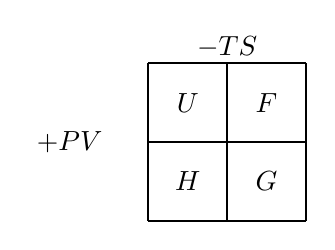
\begin{tikzpicture}[thick]
\draw (0,0) -- (2,0);
\draw (0,1) -- (2,1);
\draw (0,2) -- (2,2);
\draw (0,0) -- (0,2);
\draw (1,0) -- (1,2);
\draw (2,0) -- (2,2);
\node at (0.5,0.5) {$H$};
\node at (1.5,0.5) {$G$};
\node at (0.5,1.5) {$U$};
\node at (1.5,1.5) {$F$};
\node at (1.0,2.2) {$-TS$};
\node at (-1.0,1.0) {$+PV$};

\end{tikzpicture}
\end{figure}

\section{How to measure $\Delta{G}$}
The easiest way is,
\begin{enumerate}
\item measure the heat absorbed when the reaction takes place, $\Delta{H}$;
\item calculate $\Delta{S}$ according to the heat capacities $C_P$ and the initial/final temperature;
\item $\Delta{G}$ = $\Delta{H}$ - $T\Delta{S}$
\end{enumerate}
Consider the production of ammonia from nitrogen and hydrogen at 298 K and 1 bar, \\
\ce{N2(g) + 3H2(g) -> 2NH3(g)}\\\\
From the values of $\Delta{H}$ and S, compute $\Delta{G}$ for this reaction and check that it is consistent with the value given in the table.\\\\\\\\


\section{Electrochemical Reactions}
Consider the chemical reaction of the electrolysis of water to hydrogen and oxygen gas,\\\\
\ce{H2O(l) -> H2(g) + 1/2O2(g)}\\\\
\begin{tabular}{|c | c | c | c | c |}
\hline
Type                 &  H$_2$O(l)& H$_2$(g)& O$_2$(g)&   Total  \\\hline
$\Delta{H}$(kJ)      &  -285.8   &    0    &   0     &   285.8  \\\hline
$S$ (J/K)            &    69.9   & 130.7   & 205.1   &  -163.4  \\\hline
$P\Delta{V}$(kJ)     &           &         &         &     3.7  \\\hline
$\Delta{U}$(kJ)      &           &         &         &   282.1   \\\hline
$T\Delta{S}$(kJ)     &           &         &         &   -48.3  \\\hline
$\Delta{G}$(kJ)      &           &         &         &   237.1  \\\hline
\end{tabular}

The reverse reaction is the combustion of hydrogen gas, a reaction that might replace the internal combustion engine in future automobiles (fuel cell).
In the process of producing the electric work, the fuel cell will also dump 49 kJ of waste heat.
But the waste heat is only 17\% of heat generated from this reaction. So an ideal hydrogen fuel cell has an `efficiency' of 83\%, much better than any practical engine.


%Another good example is the electric energy output of a battery.\\\\
%\ce{Pb + PbO2 + 4H{+} + 2SO4^{2-} -> 2PbSO4 + 2H2O}\\\\
%\begin{tabular}{|c | c | c | c | c | c | c | c |}
%\hline
%Type                 &   Pb      &  PbO$_2$& H$^{+}$ &   SO$_4^{2-}$ &PbSO$_4$ & H$_2$O(l) & Total \\\hline
%$\Delta{H}$(kJ)      &           &         &         &               &         &           & \\\hline
%$S$ (J/K)            &           &         &         &               &         &           & \\\hline
%$P\Delta{V}$(kJ)     &           &         &         &               &         &           & \\\hline
%$\Delta{U}$(kJ)      &           &         &         &               &         &           &  \\\hline
%$T\Delta{S}$(kJ)     &           &         &         &               &         &           & \\\hline
%$\Delta{G}$(kJ)      &           &         &         &               &         &           & \\\hline
%\end{tabular}


\section{Thermodynamic Identities}
In the previous chapter, we already learned
\begin{equation} dU = TdS - PdV + \mu dN \end{equation}
What will happen on $H$, $F$, $G$?

\begin{equation} 
\begin{split}
dH  = &  dU + PdV + VdP   \\
    = & TdS + VdP + \mu dN 
\end{split}
\end{equation}

Similarly, we could derive that 
\begin{equation} 
\begin{split}
dF  = &  dU - (TdS + SdT)   \\
    = & -SdT  - PdV + \mu dN 
\end{split}
\end{equation}

\begin{equation} 
\begin{split}
dG  = & dF + PdV + VdP   \\
    = & -SdT + VdP + \mu dN 
\end{split}
\end{equation}

Accordingly, we can derive the partial derivatives from $G$,
\begin{equation} S   = -(\frac{\partial {G}}{\partial {T}})_{P,N} \end{equation}
\begin{equation} V   = (\frac{\partial {G}}{\partial {P}})_{T,N} \end{equation}
\begin{equation}\mu  = (\frac{\partial {G}}{\partial {N}})_{T,P} \end{equation}


\section{Maxwell Relation}
Functions encountered in physics are generally well enough behaved that their
mixed partial derivatives do not depend on which derivatives are taken first. For instance,
\begin{equation} 
                 \frac {\partial}{\partial V} (\frac{\partial U}{\partial S}) 
               = \frac {\partial}{\partial S} (\frac{\partial U}{\partial V})
\end{equation}
From the thermodynamic identities (for $U$), we can evaluate the partial derivatives,
\begin{equation} 
               (\frac{\partial T}{\partial V})_S
               = -(\frac{\partial P}{\partial S})_V
\end{equation}
Similarly, we apply it on $H$,$F$,$G$,
\begin{equation} \frac {\partial}{\partial P} (\frac{\partial H}{\partial S}) 
               = \frac {\partial}{\partial S} (\frac{\partial H}{\partial P})
               ~~~ \rightarrow ~~~~
                (\frac{\partial T}{\partial P})_S
               = (\frac{\partial V}{\partial S})_P
\end{equation}
\begin{equation} \frac {\partial}{\partial V} (\frac{\partial F}{\partial T}) 
               = \frac {\partial}{\partial T} (\frac{\partial F}{\partial V})
               ~~~ \rightarrow ~~~~
                (\frac{\partial S}{\partial V})_T
               = (\frac{\partial P}{\partial T})_V
\end{equation}
\begin{equation} \frac {\partial}{\partial P} (\frac{\partial G}{\partial T}) 
               = \frac {\partial}{\partial T} (\frac{\partial G}{\partial P})
               ~~~ \rightarrow ~~~~
                (\frac{\partial S}{\partial P})_T
               = -(\frac{\partial V}{\partial T})_P
\end{equation}

These are {\bf Maxwell relations}. It is useful because it could quantify the changes of 
entropy which are not directly measurable, in terms of measurable quantities like $T,V,P$.
Here let me just give some of its applications.
The thermal expansion coefficient is defined as follows,
\begin{equation}
\beta = \frac{\Delta{V}/V}{\Delta{T}} = -\frac{1}{V}(\frac{\partial V}{\partial T})_P
\end{equation}
Plugging in the Maxwell relation,
\begin{equation}
\beta = \frac{1}{V}(\frac{\partial V}{\partial T})_P 
      = \frac{1}{V}(\frac{\partial S}{\partial P})_T 
\end{equation}

According to the 3rd law, entropy approaches to 0 or some constant regardless of $P$. Hence $\beta$ = 0 when $T$ goes to 0.

Now let's dig into the difference between $C_V$ and $C_P$
\begin{equation}
dS = (\frac{\partial{S}}{\partial{T}})_V dT + (\frac{\partial{S}}{\partial{V}})_T dV
\end{equation}

\begin{equation}
dV = (\frac{\partial{V}}{\partial{T}})_p dT + (\frac{\partial{V}}{\partial{P}})_T dP
\end{equation}

\begin{equation}
(dS)_P = (\frac{\partial{S}}{\partial{T}})_V dT + (\frac{\partial{S}}{\partial{V}})_T (\frac{\partial{V}}{\partial T})_P dT
\end{equation}
That is,
\begin{equation}
(\frac{\partial S}{\partial T})_P = (\frac{\partial{S}}{\partial{T}})_V + (\frac{\partial{S}}{\partial{V}})_T (\frac{\partial{V}}{\partial T})_P
\end{equation}

\begin{equation}
C_P = C_V + T(\frac{\partial{S}}{\partial{V}})_T (\frac{\partial{V}}{\partial T})_P
\end{equation}

\begin{equation}
C_P = C_V + T(\frac{\partial{P}}{\partial{T}})_V (\frac{\partial{V}}{\partial T})_P
\end{equation}

from problem 1.46,
\begin{equation}
(\frac{\partial{P}}{\partial{T}})_V = -\frac{(\partial{V}/{\partial T})_P}{(\partial{V}/{\partial P})_T}
\end{equation}

Therefore,
\begin{equation}
C_P = C_V - T(\frac{\partial{V}}{\partial{T}})^2_P / (\frac{\partial{V}}{\partial P})_T
\end{equation}

Recall the definition of $\beta$ and $\kappa$
\begin{equation}
\beta = \frac{1}{V}(\frac{\partial{V}}{\partial{T}})_P;~~~~~~ \kappa_T = -\frac{1}{V}(\frac{\partial{V}}{\partial{P}})_T
\end{equation}

\begin{equation}
C_P - C_V = -T(\beta V)^2/(-\kappa_T V) = \frac{TV\beta^2}{\kappa_T}
\end{equation}



